% GripCheck design and verification report, GC-TR-002 Rev 1.0
% Build:  tectonic gripcheck_report.tex      (or upload this folder to Overleaf, compiler XeLaTeX)
\documentclass[10pt,a4paper]{article}

\usepackage[margin=2.1cm,headheight=14pt]{geometry}
\usepackage{fontspec}
\usepackage{unicode-math}
\setmainfont{texgyretermes}[Extension=.otf,UprightFont=*-regular,BoldFont=*-bold,ItalicFont=*-italic,BoldItalicFont=*-bolditalic]
\setsansfont{texgyreheros}[Extension=.otf,UprightFont=*-regular,BoldFont=*-bold,ItalicFont=*-italic,BoldItalicFont=*-bolditalic]
\setmonofont{texgyrecursor}[Extension=.otf,UprightFont=*-regular,BoldFont=*-bold,ItalicFont=*-italic,BoldItalicFont=*-bolditalic]
\setmathfont{texgyretermes-math.otf}
\usepackage{microtype}
\usepackage{graphicx}
\usepackage{booktabs}
\usepackage{tabularx}
\usepackage{array}
\usepackage{longtable}
\usepackage{float}
\usepackage{xcolor}
\usepackage{tikz}
\usetikzlibrary{arrows.meta,positioning,fit,calc}
\usepackage[font=small,labelfont=bf,skip=4pt]{caption}
\usepackage{enumitem}
\usepackage{fancyhdr}
\usepackage{lastpage}
\usepackage{titlesec}
\usepackage[hidelinks]{hyperref}

\graphicspath{{figures/}}
\setlist{itemsep=1pt,topsep=3pt}
\renewcommand{\arraystretch}{1.18}
\newcolumntype{L}{>{\raggedright\arraybackslash}X}
\newcolumntype{P}[1]{>{\raggedright\arraybackslash}p{#1}}

\definecolor{accent}{HTML}{1F4E79}
\definecolor{cellgreen}{HTML}{229E89}
\definecolor{soft}{HTML}{EEF2F6}
\definecolor{warn}{HTML}{9A3412}

\titleformat{\section}{\large\bfseries\sffamily\color{accent}}{\thesection}{0.6em}{}
\titleformat{\subsection}{\normalsize\bfseries\sffamily}{\thesubsection}{0.5em}{}
\titlespacing*{\section}{0pt}{12pt}{5pt}
\titlespacing*{\subsection}{0pt}{8pt}{3pt}

\newcommand{\docno}{GC-TR-002}
\newcommand{\docrev}{Rev.\ 1.0}
\pagestyle{fancy}
\fancyhf{}
\fancyhead[L]{\small\sffamily GripCheck Design and Verification Report}
\fancyhead[R]{\small\sffamily \docno\ \,·\, \docrev}
\fancyfoot[L]{\footnotesize Educational project. Not a medical device and not for diagnosis.}
\fancyfoot[R]{\footnotesize Page \thepage\ of \pageref{LastPage}}
\renewcommand{\headrulewidth}{0.4pt}

% Evidence classes, used in every status column
\newcommand{\meas}{\textbf{Measured}}
\newcommand{\cadan}{CAD analysis}
\newcommand{\simul}{Simulation}
\newcommand{\swt}{Software test}
\newcommand{\rep}{\textit{Reported, not recorded}}
\newcommand{\nt}{\textcolor{warn}{Not tested}}

% Photo placeholder: id, height, what to photograph
\newcommand{\photoplaceholder}[3]{%
  \begin{tikzpicture}
    \node[draw=accent!70,dashed,line width=0.8pt,fill=soft,rounded corners=3pt,
          minimum width=0.92\linewidth,minimum height=#2,text width=0.8\linewidth,align=center]
      {{\sffamily\bfseries\color{accent} PHOTO PLACEHOLDER #1}\\[4pt]\small #3};
  \end{tikzpicture}}

\begin{document}

% ------------------------------------------------------------------ title page
\thispagestyle{fancy}
\begin{center}
  {\sffamily\small\color{accent} BIOMEDICAL ENGINEERING PROJECT · TECHNICAL REPORT}\\[10pt]
  {\LARGE\bfseries GripCheck: A Low-Cost Load-Cell Grip Dynamometer\\[2pt] with Force-Time Analysis}\\[8pt]
  {\large Design and Verification Report}\\[10pt]
  Thomas Kim · Samuel Koo\\
  University of Waterloo · 23 November 2026
\end{center}

\vspace{6pt}
\noindent
\begin{tabularx}{\linewidth}{@{}>{\bfseries}p{3.6cm}L>{\bfseries}p{3.2cm}L@{}}
\toprule
Document number & \docno & Revision & 1.0 \\
Hardware & v4.2 Jamar-style, as printed (v3 reference build) & Firmware & v1.0; \texttt{SIGN = +1} change pending verification \\
Software & Commit \texttt{51e9189} & Status & Verification in progress \\
Classification & Educational prototype; no regulatory claim & Supersedes & GC-TR-002 Rev.\ 0.9 \\
\bottomrule
\end{tabularx}

\vspace{8pt}
\noindent\textbf{Approval}\par\smallskip
\noindent
\begin{tabularx}{\linewidth}{@{}p{2.6cm}p{3.6cm}p{4.2cm}L@{}}
\toprule
Role & Name & Responsibility & Signature / date \\
\midrule
Prepared by & Thomas Kim & Hardware, CAD, firmware, calibration & \\[4pt]
Reviewed by & Samuel Koo & Analysis software & \\[4pt]
Approved by & \textit{[name]} & Course instructor or supervisor & \\[4pt]
\bottomrule
\end{tabularx}

\vspace{8pt}
\noindent\textbf{Revision history}\par\smallskip
\noindent
\begin{tabularx}{\linewidth}{@{}p{1.3cm}p{2.3cm}L@{}}
\toprule
Rev. & Date & Change \\
\midrule
0.9 & 2026-11-23 & Draft status report for the v3 hardware. \\
1.0 & 2026-11-23 & Restructured as a design and verification report. Adds the v4.2 Jamar-style design, its CAD verification and first device findings; risk summary; standards assessment; verification records under test IDs; figure and media plan. \\
\bottomrule
\end{tabularx}

\vspace{10pt}
\begin{abstract}
\noindent Clinical grip dynamometers such as the Jamar report only peak force, which discards how quickly force rises and how well it is held. GripCheck is a handheld dynamometer in which all squeeze force passes through a single 100 kg single-point load cell, read by an HX711 24-bit converter and an Arduino Nano, and analysed in a browser or desktop application that administers a standardised protocol and reports peak force, time to peak, rate of force development (RFD) and fatigue index against published norms. The design has passed through four iterations. The current v4.2 Jamar-style frame, with five keyed handle settings, passes 53 of 53 automated geometry checks and has been printed and assembled. The signal chain has been demonstrated on hardware, rest noise is about ±70 counts (about 2 g), and 165 of 165 automated software tests pass. The device has not yet been calibrated against weighed masses, so its accuracy and usable range are unverified. Calibration with a held-out check load is the next milestone, and its protocol and acceptance criteria are fixed in this report before testing.
\end{abstract}

\noindent\textbf{Index terms:} force-time curve, grip strength, HX711, load cell, rate of force development, design verification.

\medskip
\noindent\fcolorbox{accent!40}{soft}{\parbox{\dimexpr\linewidth-2\fboxsep-2\fboxrule}{\small
\textbf{Key results.}
(1) Signal chain demonstrated end to end on hardware [\meas].
(2) v4.2 frame: 0.0000\,mm$^3$ interference across 10 part pairs, 17.1\,mm of free finger travel before any contact, and a keyed palm seat that carries the load at all five settings after 0.35\,mm [\cadan].
(3) A sign nonconformance on the first v4.2 squeeze was found, explained and controlled the same day.
(4) 165 of 165 software tests pass, including Python–TypeScript parity [\swt].
(5) Zero-phase filtering did not reduce RFD error in 300 simulated trials [\simul].
(6) Estimated parts cost CAD\,89.
\textbf{Force accuracy: not yet tested.}}}

\newpage
\tableofcontents
\newpage

% ------------------------------------------------------------------ 1
\section{Purpose, scope and conventions}

This report records the design inputs, design outputs, design reviews, risk controls and verification evidence for GripCheck at the end of the prototype phase. It covers the v4.2 Jamar-style hardware as printed, the v3 split-grip reference build, the firmware, and the GripCheck analysis software and website. Clinical validation, manufacturing and regulatory submission are out of scope.

\subsection{Evidence classes}
Every result carries one evidence class. A result is never presented as stronger evidence than its class.

\smallskip\noindent
\begin{tabularx}{\linewidth}{@{}p{3.6cm}L@{}}
\toprule
Class & Meaning \\
\midrule
\meas & Physical test on real hardware, with a dated build-log entry. \\
\cadan & Computed from the released CAD geometry. Says nothing about strength, deflection or fit of printed parts. \\
\simul & Synthetic data with known ground truth. Shows the arithmetic, not the device. \\
\swt & Automated test of the software against known answers. \\
\rep & Observed by a team member but values not captured. Not acceptable as verification. \\
\nt & No evidence. \\
\bottomrule
\end{tabularx}

\smallskip
Force is in kilograms-force (kg); 1 kg = 9.81 N. Mass plates are specified in pounds (lb) and converted with 1 lb = 0.45359 kg.

\subsection{Reference documents}
\noindent
\begin{tabularx}{\linewidth}{@{}p{5.6cm}L@{}}
\toprule
Document & Content \\
\midrule
\texttt{docs/01\_design\_process.md} & Original requirements and concept selection \\
\texttt{docs/06\_build\_log.md} & Dated build log: every physical test in this report \\
\texttt{docs/08\_verification\_checklist.md} & Inspection and test checklist \\
\texttt{docs/15\_calibration\_v4\_2.md} & Proof-load and calibration protocol for v4.2 (VT-09, VT-10) \\
\texttt{cad/evidence\_v4\_2/} & Geometry checker, report (53/53) and printed-part inspection sheet \\
\texttt{cad/baseline\_reconciliation/} & v4.1 to v4.2 design review and annotated holding view \\
\bottomrule
\end{tabularx}

\subsection{Standards and guidance}
GripCheck follows two clinical references and borrows the structure of several device and metrology standards. It claims conformity with none of them. Table~\ref{tab:standards} states the level of use and what conformity would still require.

\begin{table}[H]
\centering\small
\caption{Standards and guidance: level of use}\label{tab:standards}
\begin{tabularx}{\linewidth}{@{}P{3.7cm}P{2.0cm}LL@{}}
\toprule
Standard or guidance & Level & How it is used here & Conformity would still require \\
\midrule
ASHT clinical assessment recommendations, grip [4] & Followed & Seated, shoulder adducted, elbow 90°, forearm neutral, handle position 2, three trials, fixed instructions; built into both applications & A trained tester; agreement study against a Jamar (Section~\ref{sec:open}) \\
Dodds et al.\ 2014 norms [1] & Followed & Age- and sex-specific centile reference & Not applicable (a dataset) \\
ISO 13485:2016 §7.3 and 21 CFR 820 (QMSR) [5,6] & Structure only & Design inputs, outputs, reviews, verification and this report's layout & A quality management system, controlled documents, signed reviews \\
ISO 14971:2019 [7] & Structure only & Hazard, cause, harm, control and verification chain (Section~\ref{sec:risk}) & Risk management plan, probability estimates, benefit–risk review, post-production monitoring \\
ISO 376 and ASTM E74 [8,9] & Method only & Ascending and descending series, repeated runs, held-out check load (VT-10) & Traceable reference masses, temperature record, full series count, classification \\
JCGM 100:2008 (GUM) [3] & Method only & Uncertainty stated with every force figure; budget to follow calibration & A full uncertainty budget \\
IEC 62304 [10] & Practices only & Version control, reviewed merges, unit and parity tests on every change & Safety classification, architecture and problem-resolution records \\
IEC 60601-1, ISO 10993-1 [11,12] & Out of scope & USB 5 V, enclosed electronics; brief skin contact with PETG & Accredited electrical testing; biological evaluation \\
\bottomrule
\end{tabularx}
\end{table}

\subsection{Abbreviations}
ADC, analogue-to-digital converter; ASHT, American Society of Hand Therapists; CAD, computer-aided design (and Canadian dollars where a cost is given); GUM, Guide to the Expression of Uncertainty in Measurement; PETG, polyethylene terephthalate glycol; RFD, rate of force development; VT, verification test.

% ------------------------------------------------------------------ 2
\section{Current status}

\begin{table}[H]
\centering\small
\caption{Status of the questions that decide whether the device measures grip force}
\begin{tabularx}{\linewidth}{@{}P{3.6cm}LP{2.4cm}P{3.3cm}@{}}
\toprule
Question & Evidence & Class & Needed to close \\
\midrule
Does the load cell fit its mount? & Fit coupon on the delivered cell (VT-01); v4.2 assembled on it (VT-06) & \meas & Photograph linked \\
Does a squeeze produce a signal? & Bench (VT-02), v3 assembled (VT-03), v4.2 assembled (VT-06) & \meas; VT-03 \rep & Raw logs with peak and return values \\
Does a squeeze read positive on v4.2? & Reads negative with \texttt{SIGN = -1} (VT-06); firmware changed & \meas{} (finding) & Upload and direction check \\
Can force bypass the cell on v4.2? & Interference and free-travel checks (VT-05) & \cadan & Gap inspection on the assembled part \\
Is force measured accurately? & Datasheet scale factor only & \nt & VT-10 calibration and check load \\
Do the printed parts hold the load? & None & \nt & VT-09 proof load \\
Is the analysis computed as defined? & 165 automated tests (VT-11) & \swt & Faulty-trial end-to-end tests \\
Are real faulty trials detected? & Classifier on synthetic curves & \simul & Labelled device recordings \\
\bottomrule
\end{tabularx}
\end{table}

% ------------------------------------------------------------------ 3
\section{Device description and intended use}

The user squeezes two handles together. The palm bar is fixed to a printed C-frame; the finger part is bolted only to the free end of a single-point load cell whose other end is bolted to the frame, and an air gap separates the finger part from every other part. Squeeze force can therefore reach the frame only by bending the cell. The HX711 digitises the bridge signal at 10 samples/s and the Nano streams \texttt{t\_ms,raw,net,force\_kg} over USB.

\begin{figure}[H]
\centering
\begin{minipage}[b]{0.43\linewidth}\centering
  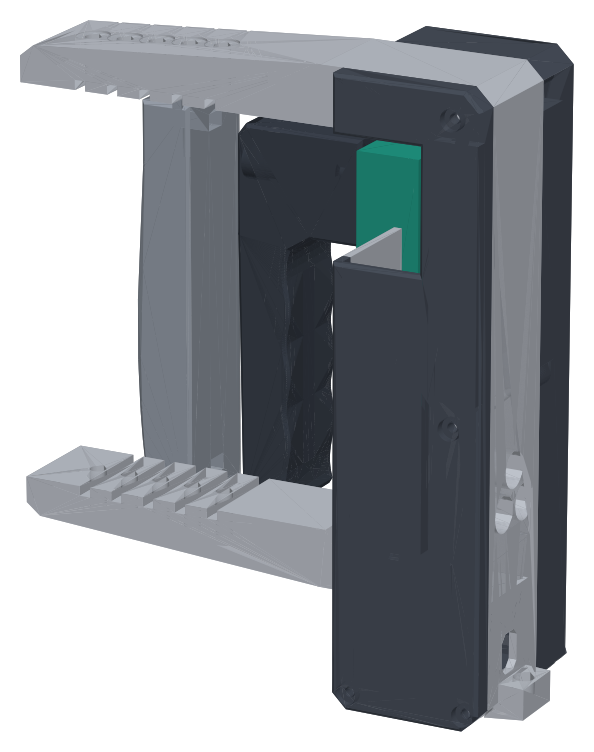
\includegraphics[width=\linewidth]{v42_render.png}\\[-2pt]
  {\small (a) Assembly}
\end{minipage}\hfill
\begin{minipage}[b]{0.43\linewidth}\centering
  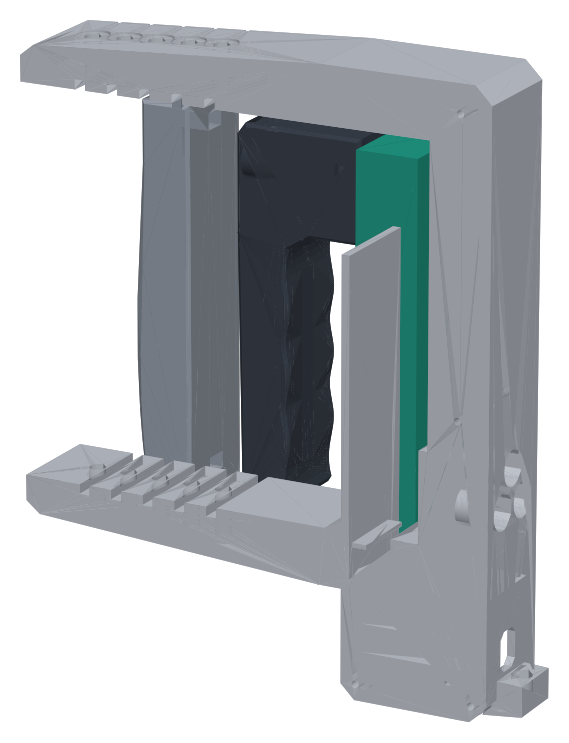
\includegraphics[width=\linewidth]{v42_open.png}\\[-2pt]
  {\small (b) Pod cover and cell guard hidden}
\end{minipage}
\caption{v4.2 Jamar-style design, rendered from the released print STLs (CAD model, not a photograph). Frame and palm bar (light grey), finger part (dark), load cell (green).}
\label{fig:v42}
\end{figure}

\begin{table}[H]
\centering\small
\caption{v4.2 key parameters (from the released CAD unless stated)}
\begin{tabularx}{\linewidth}{@{}P{5.2cm}L@{}}
\toprule
Parameter & Value \\
\midrule
Load cell & CZL601 single-point parallel beam, 100 kg, 2.0 mV/V, full bridge; delivered part measured 130 × 40 × 22 mm, three M6 holes per end [\meas] \\
Signal chain & HX711 24-bit ADC, gain 128, 10 samples/s; Arduino Nano (ATmega328P); USB serial 115\,200 baud \\
Overall size & 181 × 67 × 214 mm \\
Handle settings & 5, at a 12 mm pitch; outer span 44–92 mm; grip span 54.0–54.5 mm at setting 2 \\
Four-finger window & about 88 mm; fingertip pocket 21.5 mm \\
Finger-part free travel & 17.1 mm before contact with any fixed part \\
Palm bar seating & Bears on a keyed seat after 0.35 mm at all settings; M5 bolts locate, they do not carry load \\
Cell guard & 3.2 mm air gap to the cell flank \\
Material & PETG, printed flat without supports \\
Operating limit & 34 kg (75 lb), pending proof load \\
\bottomrule
\end{tabularx}
\end{table}

\begin{figure}[H]
\centering
\photoplaceholder{P1}{4.2cm}{v4.2 as built. Three-quarter view on a plain background, a ruler in frame for scale, same angle as Figure~\ref{fig:v42}a.}\\[6pt]
\photoplaceholder{P2}{4.2cm}{Device in use in the ASHT position: seated, shoulder adducted, elbow at 90°, forearm neutral, wrist 0–30° extension. Side-on, whole arm in frame.}
\caption{Photographs to be added before release.}
\end{figure}

\paragraph{Intended use.} Measurement of peak and sustained grip force in an educational or research-practice setting, using a standardised protocol and comparison with published normative centiles.

\paragraph{Not intended for.} Diagnosis, screening or any clinical decision; loads above 34 kg until proof-loaded; reporting forces as calibrated before VT-10 is complete.

% ------------------------------------------------------------------ 4
\section{Design inputs}

Requirements were written before any geometry and are traced to verification in Section~\ref{sec:verif}. Methods: T = test, A = analysis, I = inspection, D = demonstration.

\begin{table}[H]
\centering\small
\caption{Requirements and status for the v4.2 hardware}\label{tab:req}
\begin{tabularx}{\linewidth}{@{}p{0.7cm}P{4.2cm}p{0.9cm}LP{2.3cm}@{}}
\toprule
ID & Requirement & Method & Evidence to date & Status \\
\midrule
R1 & Measure grip force over a stated, validated range (target 0–30 kg minimum) & T & None. 100 kg is the sensor rating, not a device range & \nt \\
R2 & Error within an agreed target after calibration & T & None. Target fixed in Section~\ref{sec:vt10} before testing & \nt \\
R3 & No load path around the load cell & A, I & 0.0000 mm$^3$ interference, 10 part pairs; 17.1 mm free travel (VT-05) & \cadan{} only \\
R4 & Adjustable grip span covering adult hands; grip span 48–60 mm at the default setting & I & 5 settings, 44–92 mm outer span; 54.0–54.5 mm at setting 2 & \cadan{} only \\
R5 & Sampling $\geq$ 10 samples/s & T & HX711 at 10 samples/s (VT-02) & Met; too slow for RFD \\
R6 & Calibration loads the cell along the squeeze path & A & Strap over the finger bar, frame supported, device inverted (VT-10 protocol) & Procedure only \\
R7 & No conductive path from any grip surface to the circuit & T & None & \nt \\
R8 & No overload of the cell in use & A & Cell safe overload 120 kg; highest 90th-centile grip in the norms 64 kg [1]; no mechanical stop & Sensor rating only \\
R9 & All structural parts print flat without supports on a 240 × 240 mm bed & A, D & Watertight STLs and bed fit (VT-05); all parts printed 2026-11-22 & Met \\
R10 & Printed parts withstand maximal effort without damage or drift & A, T & None for v4.2 & \nt \\
R11 & Reproducible from the repository (CAD, firmware, BOM, procedures) & I & STEP and STL, firmware, procedures published; v4.2 BOM and assembly guide incomplete & Partly met \\
R12 & Mount tolerates supplier variation in cell hole position & T & Fit coupon on the delivered cell (VT-01) & Met (v3) \\
R13 & Every result states its calibration status & T & Estimated-calibration banner on device data (VT-11) & Met (\swt) \\
R14 & Usable in the hand without a bench & D & v3 and v4.2 squeezed by hand (VT-03, VT-06) & Met \\
\bottomrule
\end{tabularx}
\end{table}

The original R2 target of ±2\,\% of full scale allows ±2 kg at every load, which is ±10\,\% of a 20 kg reading. That is too coarse for percentile or left/right comparisons, so a reading-relative target is set in Section~\ref{sec:vt10}.

% ------------------------------------------------------------------ 5
\section{System architecture}

\begin{figure}[H]
\centering
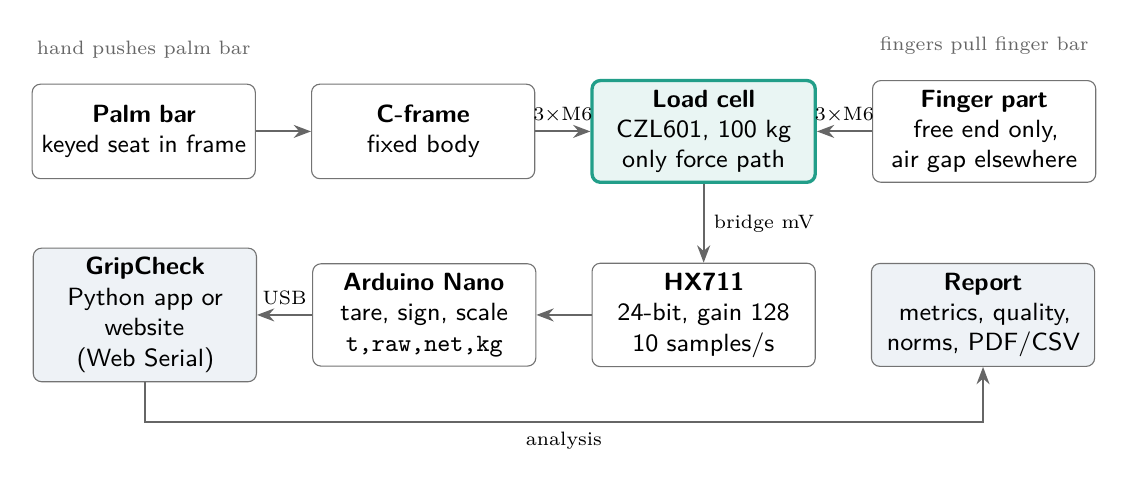
\begin{tikzpicture}[
  font=\small\sffamily, node distance=6mm and 7mm,
  blk/.style={draw=black!55, rounded corners=3pt, align=center, minimum height=12mm, text width=26mm, fill=white},
  key/.style={blk, draw=cellgreen, line width=1.2pt, fill=cellgreen!10},
  sw/.style={blk, fill=soft},
  ar/.style={-{Stealth[length=2.2mm]}, draw=black!60, line width=0.7pt}]
  \node[blk] (palm) {\textbf{Palm bar}\\ keyed seat in frame};
  \node[blk, right=of palm] (frame) {\textbf{C-frame}\\ fixed body};
  \node[key, right=of frame] (cell) {\textbf{Load cell}\\ CZL601, 100 kg\\ only force path};
  \node[blk, right=of cell] (finger) {\textbf{Finger part}\\ free end only,\\ air gap elsewhere};
  \node[blk, below=10mm of cell] (hx) {\textbf{HX711}\\ 24-bit, gain 128\\ 10 samples/s};
  \node[blk, left=of hx] (nano) {\textbf{Arduino Nano}\\ tare, sign, scale\\ \texttt{t,raw,net,kg}};
  \node[sw, left=of nano] (app) {\textbf{GripCheck}\\ Python app or\\ website (Web Serial)};
  \node[sw, right=of hx] (rep) {\textbf{Report}\\ metrics, quality,\\ norms, PDF/CSV};
  \draw[ar] (frame) -- node[above,font=\scriptsize]{3×M6} (cell);
  \draw[ar] (finger) -- node[above,font=\scriptsize]{3×M6} (cell);
  \draw[ar] (palm) -- (frame);
  \draw[ar] (cell) -- node[right,font=\scriptsize]{bridge mV} (hx);
  \draw[ar] (hx) -- (nano);
  \draw[ar] (nano) -- node[above,font=\scriptsize]{USB} (app);
  \draw[ar] (app.south) -- ++(0,-5mm) -| node[pos=0.25,below,font=\scriptsize]{analysis} (rep.south);
  \node[above=2mm of palm, font=\scriptsize, text=black!60] {hand pushes palm bar};
  \node[above=2mm of finger, font=\scriptsize, text=black!60] {fingers pull finger bar};
\end{tikzpicture}
\caption{Load path (top row) and signal chain (bottom row). The load cell is the only connection between the finger part and the rest of the device.}
\end{figure}

\begin{figure}[H]
\centering
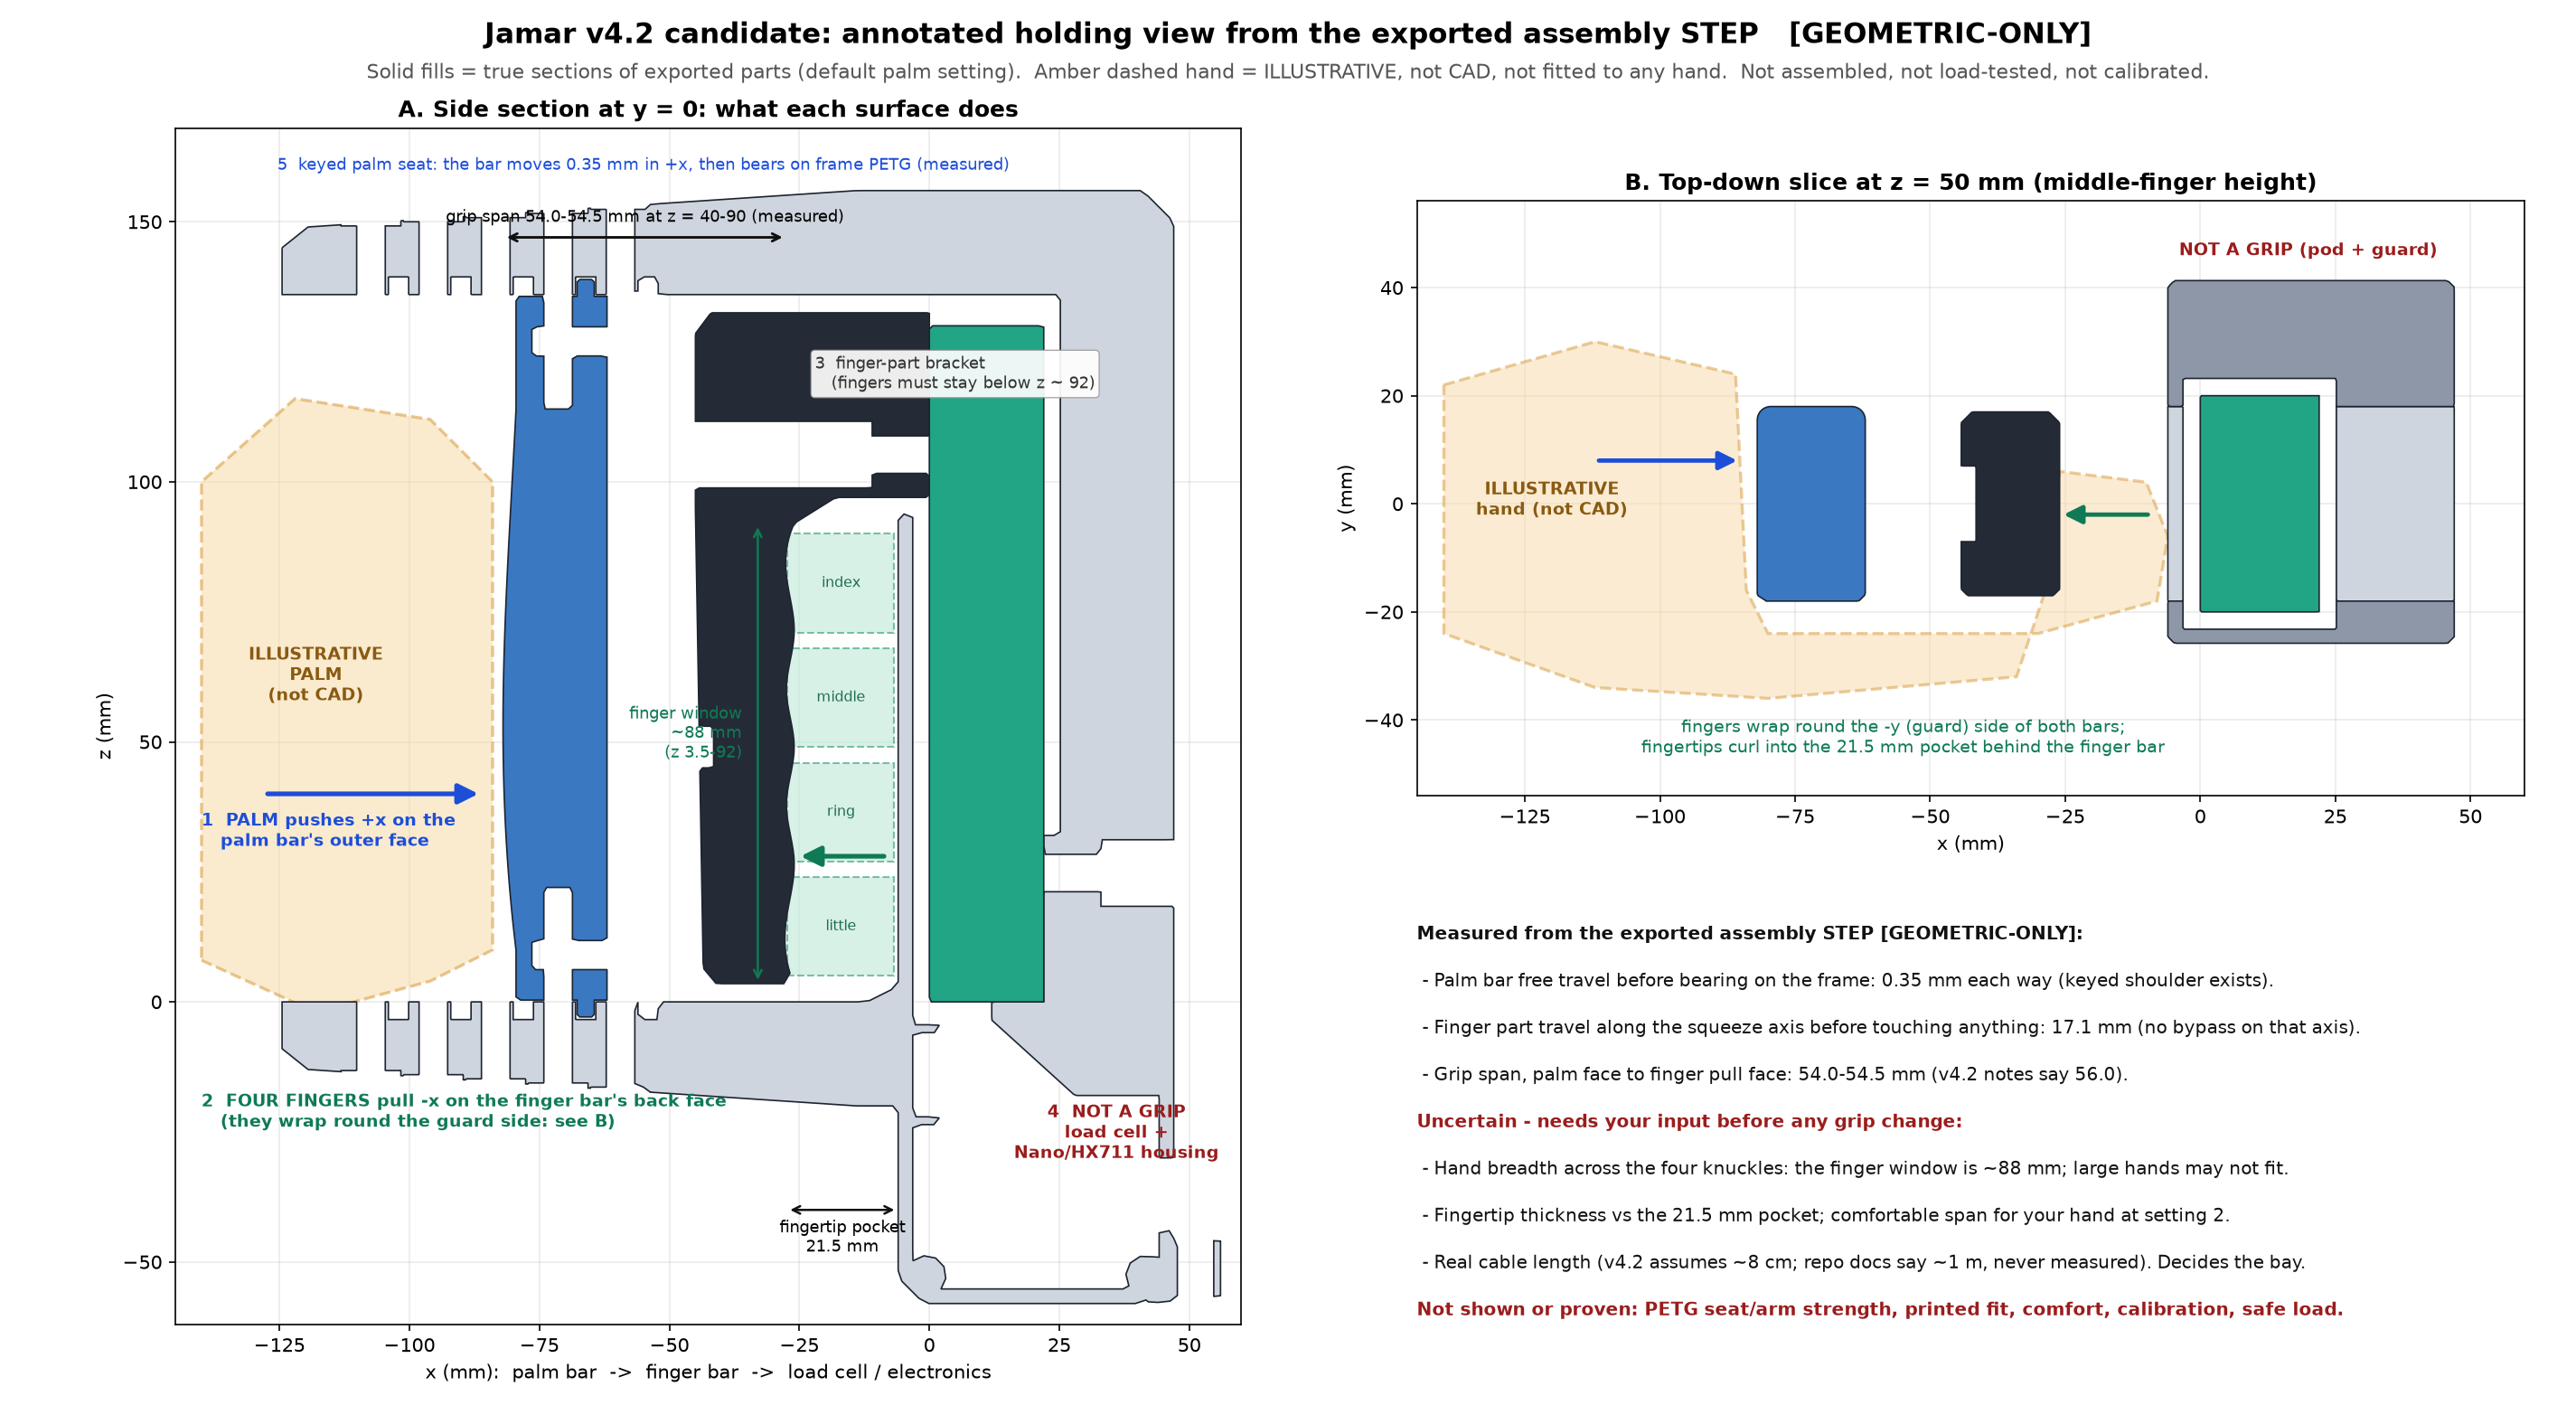
\includegraphics[width=\linewidth]{v42_holding_view.png}
\caption{v4.2 holding view from the exported assembly STEP [\cadan]. (A) Side section at y = 0: what each surface does. (B) Section at middle-finger height. The hand outline is illustrative, not fitted to a measured hand.}
\label{fig:holding}
\end{figure}

% ------------------------------------------------------------------ 6
\section{Design history and design decisions}

\begin{figure}[H]
\centering
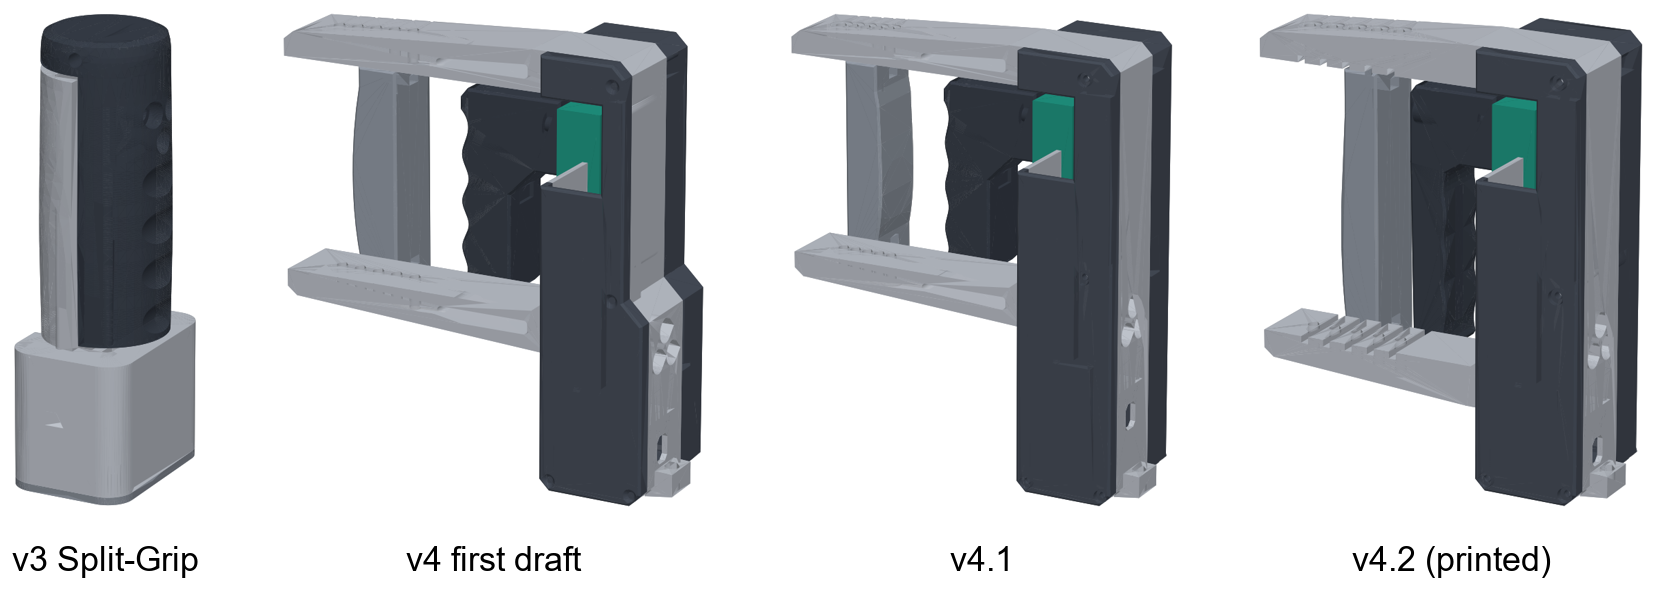
\includegraphics[width=\linewidth]{design_evolution.png}
\caption{Design iterations, rendered from each version's print STLs at the same scale and view (CAD models).}
\label{fig:evolution}
\end{figure}

\begin{table}[H]
\centering\small
\caption{Design reviews, newest first}
\begin{tabularx}{\linewidth}{@{}p{1.9cm}p{2.1cm}LP{3.1cm}@{}}
\toprule
Date & Design & Review finding & Decision \\
\midrule
2026-11-23 & v4.2, assembled & Squeeze reads negative with \texttt{SIGN = -1}: the C-frame bends the cell the opposite way to the v3 barrel & Firmware \texttt{SIGN = +1} (to verify); software direction warning added \\
2026-11-22 & v4.2 & Palm and finger contours face the squeeze; keyed palm seat; coil bay removed (17 mm shorter); 53/53 checks & Frozen; printed \\
2026-11-22 & v4.1 & Holding-view sections show the palm pad and finger scallops facing the gap and the upper bracket blocking two fingers & Superseded; never printed \\
2026-11 & v4 draft & First two-handle Jamar-style layout; support-free, 36 mm print height; captive M5 nuts & Reworked into v4.1 \\
2026-11-12 & v3 & Reads a squeeze and returns to zero; barrel handle does not match the Jamar handle convention behind the norms & Kept as reference; Jamar-style frame started \\
2026-10-16 & v3 box & Compact base chosen over a larger dish & Released for printing \\
2026-10-12 & Mount & Delivered cell 130 × 40 × 22 mm with three M6 holes per end, against a listing of 130 × 30 × 22 mm with two & Mount rebuilt from the measured part \\
\bottomrule
\end{tabularx}
\end{table}

\begin{table}[H]
\centering\small
\caption{Key design decisions}
\begin{tabularx}{\linewidth}{@{}P{3.9cm}LLP{3.3cm}@{}}
\toprule
Decision & Expected benefit & Accepted drawback & Confirming test \\
\midrule
Two-handle Jamar-style frame, 5 settings (v4) & Matches the handle convention of the clinical norms & More parts; larger device & Agreement study against a Jamar \\
Keyed palm seat; bolts only locate (v4.2) & Load carried in bearing, not by M5 bolts in PETG & Seat strength in PETG untested & VT-09 proof load \\
Cantilevered cell; no pivot or guide pins in the load path & Fewer friction contacts, lower hysteresis & Printed frame acts as a cantilever and may flex & Ascending and descending runs (VT-10) \\
CZL601 single-point cell & Insensitive to where the hand loads the bar & Cell body sets handle size & Same mass at three strap heights \\
Finger part bolted to one cell end only, air gap elsewhere & Cell is the only force path & Any contact across the gap bypasses the cell & Gap inspection; hand vs.\ hung-load agreement \\
No mechanical overload stop & Removes a part that could not be printed accurately & No protection above the sensor rating & None; accepted for supervised use \\
HX711 at its default 10 samples/s & Lower noise; no board rework & No RFD; time to peak resolved to 100 ms & Repeat at 80 samples/s \\
Simulator emitting the firmware format & Software built before hardware & Simulated curves may not match real ones & Compare with recordings \\
Butterworth filter (4th order, 10 Hz, zero-phase) & Noise reduction without time shift & Not supported by simulation (Section~\ref{sec:sim}) & Raw vs.\ filtered RFD on device data \\
Random Forest quality check with rule fallback & Flags faulty trials for repetition & Trained on synthetic data only & Labelled device recordings \\
\bottomrule
\end{tabularx}
\end{table}

% ------------------------------------------------------------------ 7
\section{Risk management summary}\label{sec:risk}

Severity: 1 negligible, 2 minor, 3 injury. Hazards are listed by severity.

\begin{table}[H]
\centering\small
\caption{Hazards, controls and verification}
\begin{tabularx}{\linewidth}{@{}p{0.6cm}P{2.9cm}p{0.5cm}LP{3.0cm}@{}}
\toprule
ID & Hazard (cause) & Sev. & Control & Verification \\
\midrule
H1 & Printed part fractures under load (PETG strength unknown; no FEA) & 3 & 34 kg limit; staged proof load before maximal squeezes; stop at the first crack or creak & VT-09 (open) \\
H2 & Finger pinched between moving and fixed parts & 2 & Cell guard; 3.2 mm air gap; free-travel check & VT-05 [\cadan] \\
H3 & Force bypasses the cell (contact, cable, strap) & 2 & Air gap on every face; strap on the finger bar only & VT-05 [\cadan]; inspection open \\
H4 & Wrong sign hides force (frame bends the cell the other way) & 2 & Direction check before use; warning below $-2$ kg with a Reverse control & VT-06 finding; VT-11 [\swt] \\
H5 & Uncalibrated force trusted (datasheet factor, about ±10\,\%) & 2 & Banner on every device result; the word ``calibrated'' withheld & VT-11 [\swt] \\
H6 & Re-zero under load (Nano resets when the port opens) & 2 & Logger started once per session; restart detection & VT-11 [\simul] \\
H7 & Electric shock & 1 & USB 5 V only; enclosed electronics & R7 continuity (open) \\
H8 & Peak over-read (zero-phase filter rings on a fast rise) & 1 & Report raw peak; move to 80 samples/s & Simulation: up to 2.1\,\% at 10 samples/s \\
H9 & Cable damage in the pod (real length unknown; CAD assumes about 8 cm) & 1 & Measure before closing the pod & Open \\
\bottomrule
\end{tabularx}
\end{table}

% ------------------------------------------------------------------ 8
\section{Verification records}\label{sec:verif}

Fields not captured at the time are marked ``not recorded''. A reported observation without values is listed for completeness and is not counted as verification.

\begin{small}
\begin{longtable}{@{}p{1.1cm}P{3.3cm}p{1.6cm}P{5.2cm}P{2.6cm}@{}}
\caption{Verification test records}\\
\toprule
ID & Item and criterion & Date & Observed & Result (class) \\
\midrule
\endfirsthead
\toprule
ID & Item and criterion & Date & Observed & Result (class) \\
\midrule
\endhead
VT-01 & Fit coupon on the delivered cell. Cell seats; bolts pass the slots & 2026-10-14 & Pass. Photograph not linked & Pass (\meas) \\
VT-02 & Bench signal chain. Reading changes by $\geq$ 10\,000 counts when pressed and returns on release & 2026-11-06 & Rest about +52\,400 counts, noise about ±70 counts; press drove the reading negative and it returned on release; upward drift during warm-up & Pass (\meas) \\
VT-03 & Assembled v3 squeeze. Reading rises on squeeze and returns to zero & 2026-11-12 & Pass reported; peak and return values not recorded & Demonstrated (\rep) \\
VT-04 & v3 direction check. Squeeze gives positive \texttt{net} & 2026-11-12 & Positive with \texttt{SIGN = -1} & Pass (\meas) \\
VT-05 & v4.2 geometry, 53 automated checks (solids, watertight STLs, bed fit, interference, free travel, keyed seat at 5 settings, source rebuild) & 2026-11-22 & 53 of 53 pass & Pass (\cadan) \\
VT-06 & v4.2 assembled, first squeeze. Reading rises on squeeze & 2026-11-23 & Responds to squeeze but reads negative with \texttt{SIGN = -1}; chart drew nothing because axes start at 0 kg. Firmware changed to \texttt{SIGN = +1}, not yet uploaded & Nonconformance; corrective action open (\meas) \\
VT-07 & v4.2 informal check loads & 2026-11-23 & Readings reported to agree with the datasheet prediction for 10–65 lb; individual values, hanger mass and run structure not recorded & Not accepted as calibration (\rep) \\
VT-08 & Printed-part inspection: 13 features against accept ranges & — & Inspection sheet prepared & \nt \\
VT-09 & Proof load 5 to 30 kg, 30 s steps; zero return within ±200 counts; 5 min creep at 30 kg & — & Protocol written & \nt \\
VT-10 & Calibration and held-out check load (Section~\ref{sec:vt10}) & — & Protocol and acceptance criteria fixed & \nt \\
VT-11 & Software: 91 Python and 74 TypeScript tests, including parity and a simulated device streaming $-25$ kg (warning shown; Reverse gives +25.0 kg) & 2026-11-23 & 165 of 165 pass at \texttt{51e9189} & Pass (\swt) \\
\bottomrule
\end{longtable}
\end{small}

\subsection{VT-10: calibration and check-load protocol (fixed before testing)}\label{sec:vt10}

\paragraph{Set-up.} Device inverted with the palm bar down, frame resting on two wooden blocks by its arms (never clamped), a 25 mm strap over the finger bar's back face at middle-finger height touching nothing else, hanger below. Logger started once for the whole session. Direction check first: a squeeze and a small hung mass must both give positive \texttt{net}.

\paragraph{Loading.} Every plate and the hanger weighed on a laboratory scale. Six levels (empty hanger, then 10, 25, 45, 55 and 65 lb of plates plus hanger), ascending then descending, at least two runs (three preferred), 10 s settling per step. The 35 lb plate is applied alone as a check load and is never used in the fit. Total load never exceeds 34 kg (75 lb).

\paragraph{Analysis.} Least-squares line of \texttt{net} against weighed mass (\texttt{software/calibrate.py}), with a curvature check.

\begin{table}[H]
\centering\small
\caption{VT-10 acceptance criteria}
\begin{tabularx}{\linewidth}{@{}p{0.8cm}P{4.4cm}L@{}}
\toprule
\# & Quantity & Criterion \\
\midrule
C1 & Fitted sensitivity & Within ±30\,\% of the datasheet 42\,952 counts/kg (sanity bound) \\
C2 & Calibrated range & 0 to at least 30 kg \\
C3 & Check-load error & Proposed: $\leq$ 2\,\% of reading (to be approved before testing) \\
C4–C6 & Non-linearity, hysteresis, repeatability & Reported as \% of calibrated range \\
C7 & Curvature & Straight line adequate \\
C8 & Zero return after load & Within ±200 counts \\
C9, C10 & Creep (5 min), rest noise (1 s.d.) & Reported \\
\bottomrule
\end{tabularx}
\end{table}

\begin{figure}[H]
\centering
\photoplaceholder{P3}{4cm}{VT-10 rig: device inverted on wooden blocks, strap over the finger bar, hanger and plates, laptop showing the live \texttt{net} reading. One wide shot and one close-up of the strap path.}
\caption{Calibration rig (photograph to be added).}
\end{figure}

% ------------------------------------------------------------------ 9
\section{Results}

No measurement-performance result exists yet: sensitivity, range, non-linearity, hysteresis, repeatability, drift and check-load error are untested. The results below are the evidence available at this stage.

\subsection{Measured}
\paragraph{Load cell dimensions.} The delivered cell measured 130 × 40 × 22 mm with three M6 holes per end, against a listing of 130 × 30 × 22 mm with two. The mount CAD was rebuilt from the measured part before any handle was printed. Purchased parts are now measured before dependent CAD is released.

\begin{figure}[H]
\centering
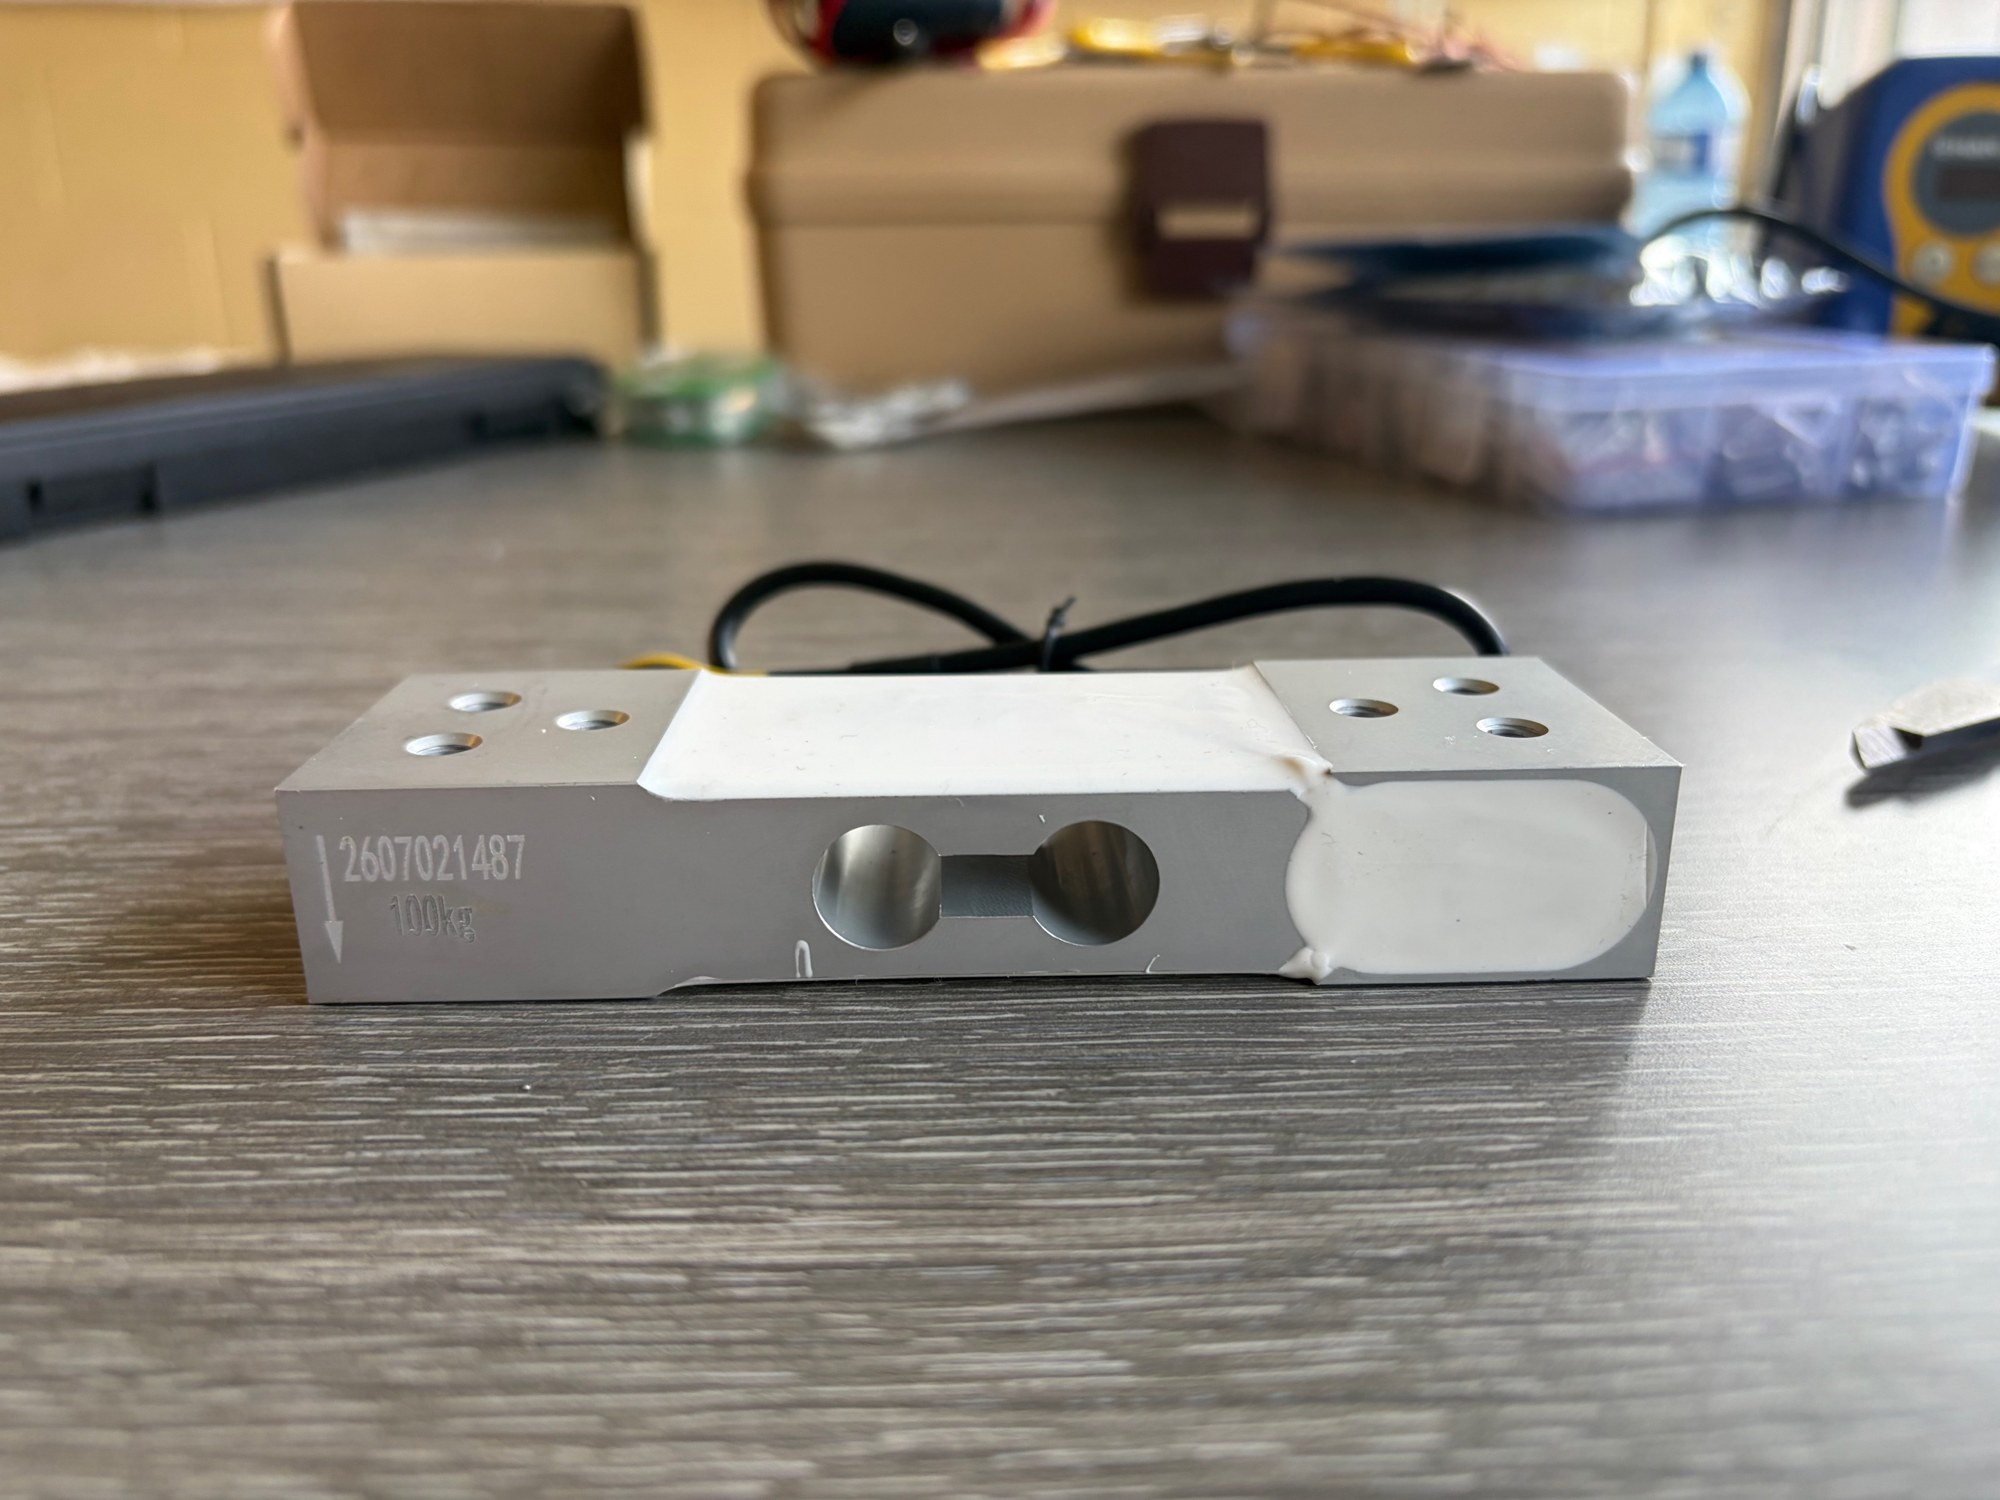
\includegraphics[width=0.55\linewidth]{load_cell_photo.jpg}
\caption{Delivered CZL601 100 kg load cell, photographed 2026-10-12.}
\end{figure}

\paragraph{Rest noise.} ±70 counts about a rest value of +52\,400 counts, about 2 g at the datasheet scale factor: negligible against trial-to-trial grip variation. Warm-up drift was observed but not quantified; it must be measured before 30 s holds are interpreted.

\paragraph{Sign on v4.2.} The same cell and firmware that read positive in the v3 barrel read negative in the v4.2 frame, because the two frames bend the cell in opposite directions. Requirement R6 (calibration along the squeeze path) exists for exactly this reason: the load path, not the sensor, sets the sign.

\subsection{Software}
All 165 automated tests pass at commit \texttt{51e9189}: 91 Python (metrics against curves with known answers, zero-phase filtering, both input formats, end-to-end protocol against a simulated serial device, calibration fitting and stream checks on a simulated cell) and 74 TypeScript, including parity with the Python reference and the direction warning. Coverage has one known gap: the simulator selects a fault type but always returns a clean curve, so no faulty trial has yet passed through the system end to end.

\begin{figure}[H]
\centering
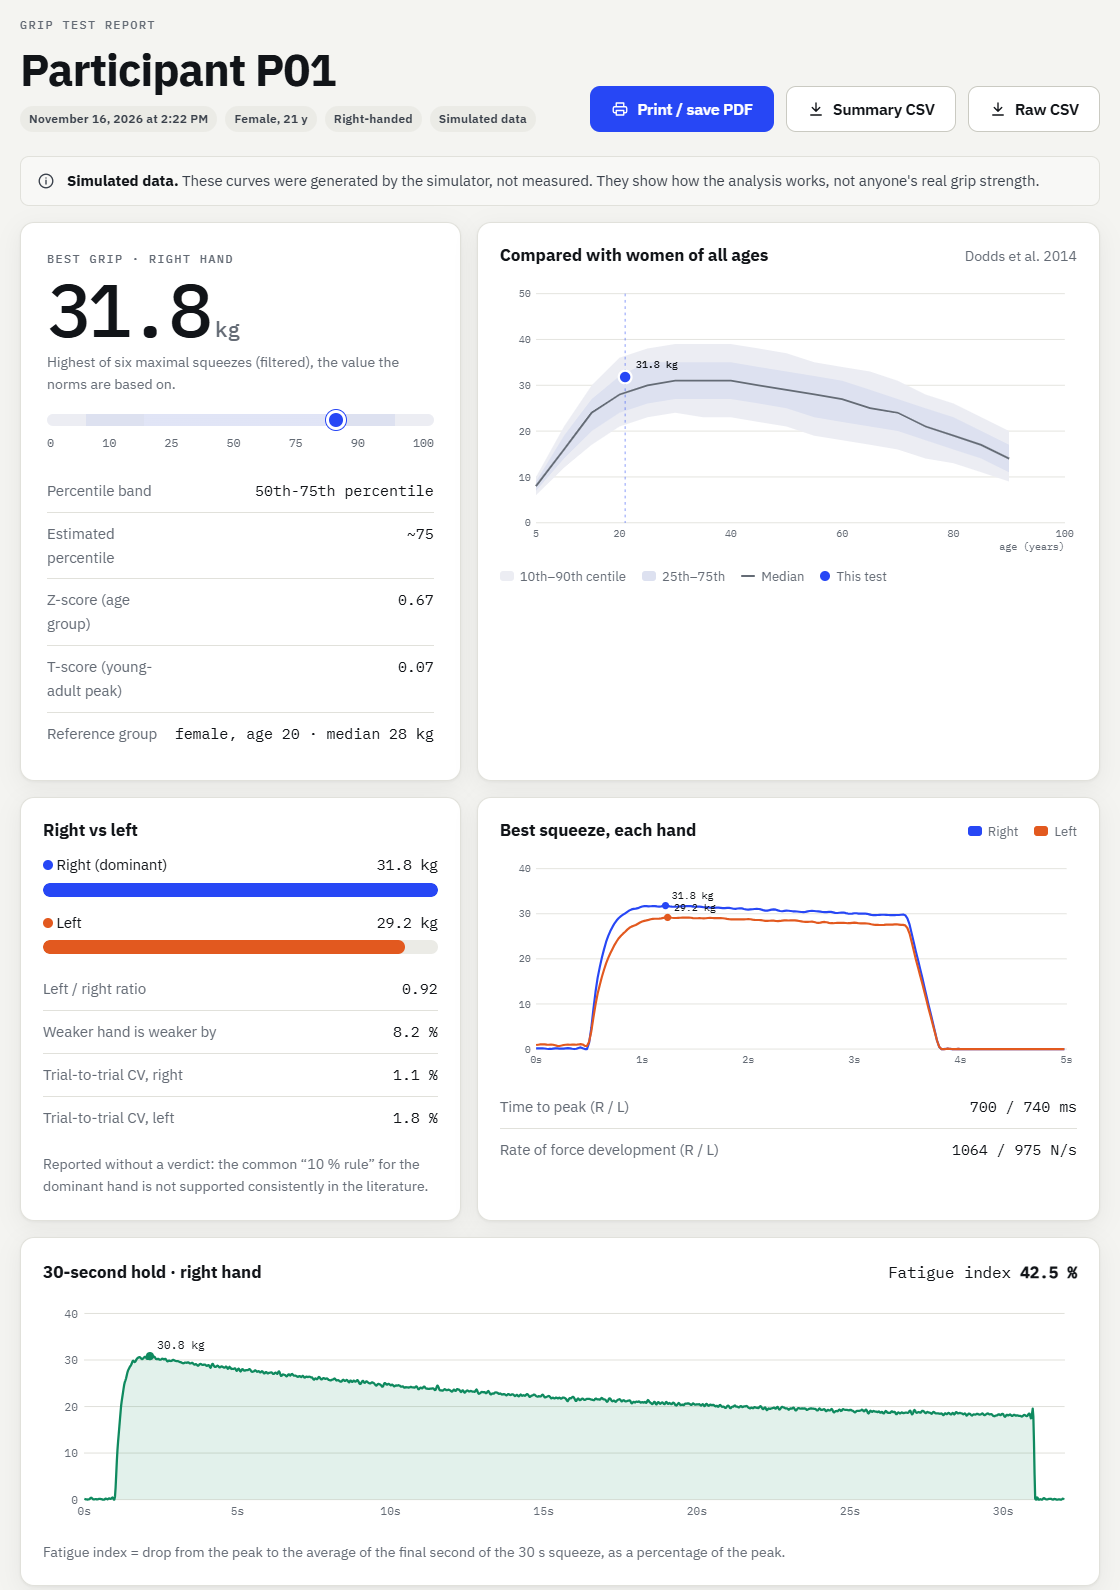
\includegraphics[width=0.62\linewidth]{web_report_simulated.png}
\caption{GripCheck website report page for a simulated session (the page labels it ``Simulated data''). Not a measurement.}
\end{figure}

\subsection{Simulation}\label{sec:sim}
\paragraph{Filter.} Over 300 simulated trials (true RFD 1\,044 N/s):

\begin{center}\small
\begin{tabular}{@{}lrr@{}}
\toprule
Signal & Mean RFD error (N/s) & Error s.d. (N/s) \\
\midrule
Raw & $-0.8$ & 21.5 \\
Butterworth, zero-phase & +13.9 & 24.7 \\
5-point moving average & +83.4 & 14.7 \\
\bottomrule
\end{tabular}
\end{center}

\begin{figure}[H]
\centering
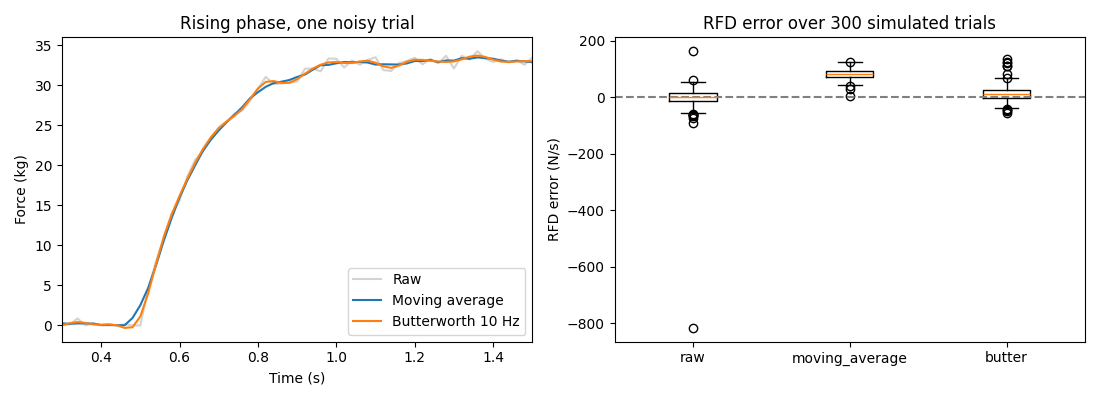
\includegraphics[width=0.9\linewidth]{filter_comparison.png}
\caption{Filter comparison on simulated trials [\simul].}
\end{figure}

Filtering did not improve either error measure under these conditions, and the zero-phase filter over-reads a fast peak by up to about 2.1\,\% at 10 samples/s (0.2\,\% at 80 samples/s). The filter choice is provisional until raw and filtered RFD are compared on device recordings.

\paragraph{Trial-quality classifier.} Trained on 2\,000 synthetic curves, the Random Forest scored 99.2\,\% on 500 held-out synthetic curves (hand-tuned rules: 92.2\,\%). This shows the model separates the simulator's shapes, not real faults. In the training data, submaximal curves differ from good ones mainly in absolute peak (21.5 vs.\ 34.3 kg), so a weak but maximal effort may be classed as submaximal; a person-relative feature, such as each peak as a fraction of that hand's best trial, should replace it.

\begin{figure}[H]
\centering
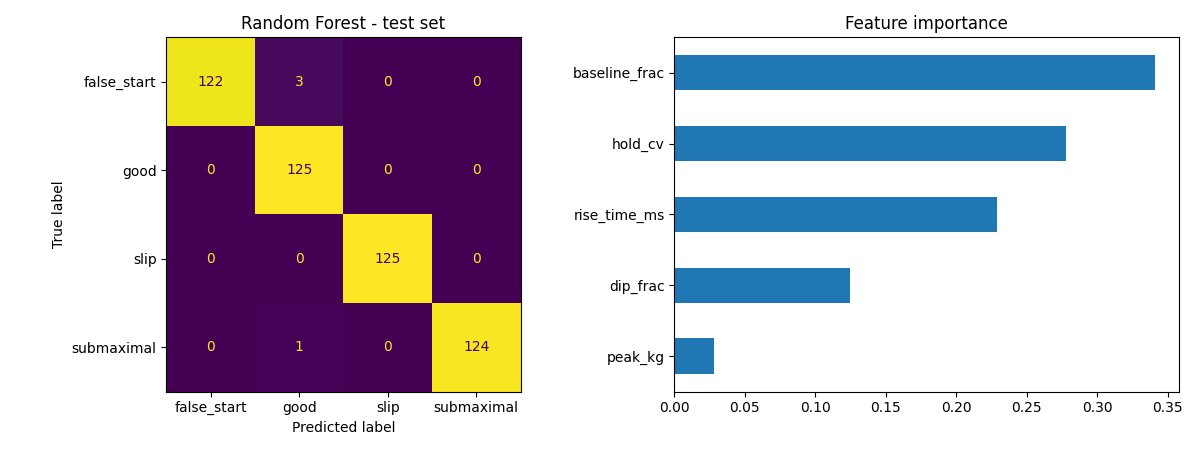
\includegraphics[width=0.9\linewidth]{quality_model.png}
\caption{Trial-quality classifier on synthetic curves [\simul].}
\end{figure}

\subsection{CAD analysis}

\begin{table}[H]
\centering\small
\caption{v4.2 geometry verification (VT-05)}
\begin{tabularx}{\linewidth}{@{}LP{5cm}@{}}
\toprule
Check & Result \\
\midrule
Each of 5 parts is one valid STEP solid; STL watertight with consistent winding; STEP and STL volumes within 1\,\% & Pass \\
Each part lies flat; parts and all 6 combined plates fit 240 × 240 mm & Pass \\
Interference between printed parts (10 pairs) & 0.0000 mm$^3$ \\
Finger-part travel toward the palm before contact & 17.1 mm \\
Palm bar travel before bearing on the keyed seat, all 5 settings & 0.35 mm \\
Source rebuilds the exported palm bar & 0.000\,\% volume difference \\
\bottomrule
\end{tabularx}
\end{table}

For v3: 0.000 mm$^3$ interference between the finger half and fixed parts, at least 3.00 mm clearance to the cell's bending zone, and replacing the round bore with a cell-shaped pocket raised the second moment of area at mid-grip from 29\,078 to 35\,756 mm$^4$ (×1.2) while nearly tripling the wall under the finger grooves (about 4 to 11.5 mm), because the added material sits near the neutral axis. None of these figures describes stress or deflection under load.

% ------------------------------------------------------------------ 10
\section{Discussion and limitations}

The prototype demonstrates the signal chain end to end on two frames; it does not yet measure force. Every quantity that depends on kilograms, including centile bands, left/right ratios and fatigue index, is illustrative until VT-10 is complete.

The most informative results so far are the three that changed the design or its status: the delivered cell's dimensions, the simulation that did not support filtering, and the v4.2 sign reversal. Test counts and classifier accuracy carry less weight, because they measure agreement between the software and its own simulator.

Further limitations:
\begin{itemize}
  \item Normative comparisons use British cohort data matched to the nearest 5-year age band [1].
  \item No finite-element analysis; strength of the keyed seat, M3 self-tapping pilots and PETG under sustained load is unproven.
  \item The 88 mm finger window has not been checked against measured hands, and the effect of load position along the bar is untested.
  \item No systematic comparison with existing low-cost or open-source dynamometers has been made.
\end{itemize}

% ------------------------------------------------------------------ 11
\section{Open issues and next milestone}\label{sec:open}

\paragraph{Next milestone: calibration and check-load verification of v4.2.} Complete when VT-08 and VT-09 pass, VT-10 meets C1–C8 with raw CSV files and the analysis commit recorded, the fitted sensitivity is committed to the firmware, and uncertainty is stated following the GUM [3].

\begin{table}[H]
\centering\small
\caption{Open issues}
\begin{tabularx}{\linewidth}{@{}P{3.5cm}p{1.9cm}LP{2.0cm}p{1.6cm}@{}}
\toprule
Issue & Status & Closed when & Owner & Due \\
\midrule
Sign on v4.2 (VT-06) & Fix made, unverified & Firmware uploaded; squeeze and hung mass both positive & T.\ Kim & \textit{[date]} \\
Proof load (R10, VT-09) & \nt & All steps pass; no cracks; zero returns & T.\ Kim & \textit{[date]} \\
Calibration and check load (R1, R2) & \nt & VT-10 complete & T.\ Kim & \textit{[date]} \\
Measurement evidence for VT-03, VT-07 & Incomplete & Raw logs linked & T.\ Kim & \textit{[date]} \\
Electrical isolation (R7) & \nt & Open circuit from every grip surface to every circuit node & T.\ Kim & \textit{[date]} \\
Cable length and pod fit & Open & Measured; pod closes without a tight bend & T.\ Kim & \textit{[date]} \\
80 samples/s acquisition & Not implemented & Logged interval $\leq$ 13 ms; noise re-measured & T.\ Kim & \textit{[date]} \\
Simulator fault defect & Open & End-to-end test per fault type fails before the fix, passes after & S.\ Koo & \textit{[date]} \\
Calibration flag in software & Waits on VT-10 & \texttt{CALIBRATION = "measured"} in both applications & S.\ Koo & \textit{[date]} \\
Classifier on real trials & \nt & Confusion matrix on labelled device data & S.\ Koo & \textit{[date]} \\
Agreement with a Jamar & Not planned in detail & Bland–Altman bias and 95\,\% limits of agreement [2]; ethics question answered first & Both & \textit{[date]} \\
\bottomrule
\end{tabularx}
\end{table}

% ------------------------------------------------------------------ 12
\section{Conclusion}

GripCheck has a verified design process and a working signal chain, but not yet a verified measurement. The v4.2 frame meets its geometric requirements, the software meets its specification on known inputs, and the first assembled squeeze exposed a sign reversal that was traced to the load path and controlled the same day. The device becomes a measuring instrument only when VT-09 and VT-10 pass; until then every force it reports is datasheet-scaled and labelled as such.

% ------------------------------------------------------------------ appendices
\appendix
\section{Bill of materials (v3, estimated)}

\begin{center}\small
\begin{tabularx}{\linewidth}{@{}p{2.6cm}Lp{0.8cm}p{2.0cm}@{}}
\toprule
Item & Specification & Qty & Est.\ cost (CAD) \\
\midrule
Load cell & CZL601, 100 kg single-point, 2.0 mV/V & 1 & 23 \\
Amplifier & HX711 24-bit breakout (4-pack) & 1 & 12 \\
Microcontroller & Arduino Nano (ATmega328P) with USB cable (3-pack) & 1 & 25 \\
Fasteners & M6 × 25 button head (6), M6 washers (6), M3 × 10 (4) & 16 & 6 \\
Printing & PETG, about 310 g at CAD 0.07/g, including fit coupon and calibration cradle & — & 23 \\
\midrule
\textbf{Total} & & & \textbf{89} \\
\bottomrule
\end{tabularx}
\end{center}
Estimates from supplier listings, to be replaced with receipts. Borrowed tools and measuring equipment are excluded. v4.2 fasteners (M5 palm-bar bolts, M3 cover and guard screws) and PETG mass are to be added.

\section{Data and code}

\begin{center}\small
\begin{tabularx}{\linewidth}{@{}p{6cm}L@{}}
\toprule
Item & Location \\
\midrule
Repository (code, CAD, firmware, documentation) & github.com/nxtkim-1/hand-dynamometer, commit \texttt{51e9189} \\
v4.2 CAD (frozen, as printed) & \texttt{cad/jamar\_v4\_2\_review/} \\
v4.2 geometry checks (VT-05) & \texttt{python cad/evidence\_v4\_2/check\_v4\_2.py} \\
Calibration fit (VT-10) & \texttt{python software/calibrate.py data/calibration\_points.csv} \\
Filter comparison & \texttt{python filters.py} \\
Classifier training and evaluation & \texttt{python train\_quality.py} \\
Test suites (VT-11) & \texttt{python -m pytest}; \texttt{npx vitest run} in \texttt{website/} \\
Build log & \texttt{docs/06\_build\_log.md} \\
Public application & gripcheck.vercel.app \\
\bottomrule
\end{tabularx}
\end{center}

\section{Figure and media list}

Photographs still to be taken. Shoot on a plain background in daylight, include a ruler where size matters, and record the date in the file name (\texttt{YYYY-MM-DD\_name.jpg}).

\begin{center}\small
\begin{tabularx}{\linewidth}{@{}p{0.8cm}LP{3.2cm}@{}}
\toprule
ID & Content & Used in \\
\midrule
P1 & v4.2 as built, three-quarter view, ruler in frame & Section 3 \\
P2 & Device held in the ASHT position, side-on & Section 3 \\
P3 & VT-10 rig, wide shot and strap close-up & Section 8 \\
P4 & Cell guard removed: air gap around the cell, paper slid through the gap & VT-08, R3 \\
P5 & Electronics pod open: Nano, HX711, cable routing & Section 3, H9 \\
P6 & Printed parts laid out before assembly, with calipers on one inspection feature & VT-08 \\
P7 & v3 assembled reference build & Section 6 \\
P8 & Live reading in GripCheck during a real squeeze (screen capture) & VT-06 \\
\bottomrule
\end{tabularx}
\end{center}

\paragraph{Supplementary video V1} (\textit{[link]}). 60–90 s demonstration: device overview, squeeze in the ASHT position with the live force trace, return to zero on release, the five handle settings, and a hung-mass check during calibration.

\begin{figure}[H]
\centering
\photoplaceholder{P4}{3.6cm}{Cell guard removed: the air gap around the load cell, with a sheet of paper slid through to show nothing touches.}\\[6pt]
\photoplaceholder{P5}{3.6cm}{Electronics pod open: Nano, HX711 and the load-cell cable route.}
\caption{Inspection photographs to be added.}
\end{figure}

% ------------------------------------------------------------------ references
\section*{References}
\addcontentsline{toc}{section}{References}
\begin{enumerate}[label={[\arabic*]},leftmargin=2.2em,itemsep=2pt]\small
\item Dodds RM, Syddall HE, Cooper R, et al. Grip strength across the life course: normative data from twelve British studies. \textit{PLoS ONE}. 2014;9(12):e113637. doi:10.1371/journal.pone.0113637
\item Bland JM, Altman DG. Statistical methods for assessing agreement between two methods of clinical measurement. \textit{The Lancet}. 1986;327(8476):307–310.
\item Joint Committee for Guides in Metrology. \textit{JCGM 100:2008, Evaluation of measurement data: Guide to the expression of uncertainty in measurement}. 2008.
\item American Society of Hand Therapists. \textit{Clinical Assessment Recommendations}, grip strength. \textit{[edition and year to be confirmed]}
\item ISO 13485:2016. Medical devices: Quality management systems: Requirements for regulatory purposes.
\item U.S. Food and Drug Administration. 21 CFR Part 820, Quality Management System Regulation.
\item ISO 14971:2019. Medical devices: Application of risk management to medical devices.
\item ISO 376. Metallic materials: Calibration of force-proving instruments used for the verification of uniaxial testing machines.
\item ASTM E74. Standard Practices for Calibration and Verification for Force-Measuring Instruments.
\item IEC 62304. Medical device software: Software life cycle processes.
\item IEC 60601-1. Medical electrical equipment: General requirements for basic safety and essential performance.
\item ISO 10993-1. Biological evaluation of medical devices: Evaluation and testing within a risk management process.
\end{enumerate}

\end{document}
